\section{Formát spustitelných souborů}
%https://en.wikipedia.org/wiki/Comparison_of_executable_file_formats
%https://dspace.vutbr.cz/xmlui/bitstream/handle/11012/53219/7141.pdf?sequence=1&isAllowed=y
%https://blog.malwarebytes.com/threat-analysis/2014/05/five-pe-analysis-tools-worth-looking-at/

%ABI vs API

% WHAT IS THIS AND HOW IT WORKS

%% Spustitelné soubory v operačních systémech
%%% srovnání atd

%% Obsah PE hlavičky

%%% WHAT IS THAT
%%% Analýza
%%% Aplikace

%%%%%
%%%%% CITACE
%%%%%

Spustitelný soubor je speciální druh souboru, který obsahuje instrukce pro provedení určité činnosti \cite{executable_lifewire}. Například se může jednat o strojový kód nebo zdrojový kód určený pro interpret. %Spustitelné soubory se oproti běžným souborům liší hlavně tím, že 

%Na rozdíl od běžných binárních (datových) souborů není spustitelné soubory 

Oproti běžným binárním souborům není v případě spustitelných souborů potřeba žádná externí aplikace k interpretovaní těchto dat. Aby bylo možné program spustit musí být formát souboru přizpůsoben operačnímu systému \cite{wiki:Executable}.

Ke spuštění programu dojde tak, že program zavaděče (anglicky loader), jež je běžně součástí operačního systému, načte program do paměti a připraví potřebné knihovny pro spuštění viz~obrázek č. \ref{fig:file_execution}.

\begin{figure}[!ht]
    \centering
    \caption{Proces spuštění souboru}
    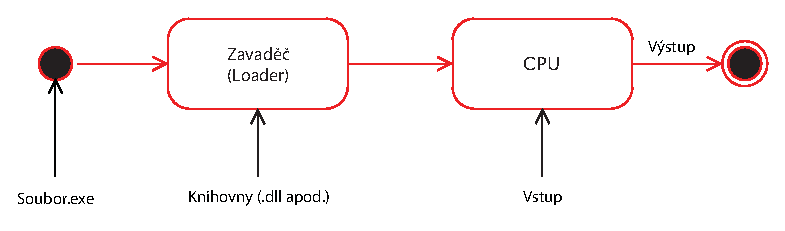
\includegraphics[width=150mm,scale=0.5]{Figures/obrazky/Execution.eps}
    \label{fig:file_execution}
\end{figure}

Aby ke spuštění mohlo vůbec dojít, musí operační systém podporovat formát spustitelného souboru na nízké úrovni  \cite{wiki:Executable}. K tomu slouží jasně definované rozhraní ABI (Application binary interface). Toto rozhraní definuje pravidla pro spolupráci strojového kódu a jádra OS. Podpora jednotného ABI na různých systémech pak umožňuje kompatibilitu zkompilované aplikace mezi různými systémy.

%https://en.wikipedia.org/wiki/Loader_(computing)
%https://en.wikipedia.org/wiki/Executable
%https://en.wikipedia.org/wiki/Application_binary_interface
%https://tristudy.com/flow-of-c-programming/

%https://cs.wikipedia.org/wiki/Zavad%C4%9B%C4%8D_(program)
%https://tristudy.com/flow-of-c-programming/

\subsection{Spustitelné soubory v OS}
% PE File, Elf, APK
%% V OS Windows PE File
%% V OS Linux ELF
%% Andorid APK

% Každý systém obsahuje jasně definované co obsahuje spustitelný soubor a 
% jaká je definovaná struktura
% v čem je rozdíl mezi systémy

%https://en.wikipedia.org/wiki/Comparison_of_executable_file_formats

Všechny operační systémy, které obsahují podporu zavedení vlastního programu, definují jeden nebo více podporovaných formátů spustitelných souborů. Tabulka č. \ref{table:executableFileformat} prezentuje některé spustitelné formáty a informace, na které platformě je můžeme najít.

%%%%% ROZDIL

\noindent
\begin{table}[H]
    \caption{Formáty spustitelných souborů (Zdroj dat \cite{wiki:Comparison_of_executable_file_formats})}
    \label{table:executableFileformat}
    
    \centering
    \begin{tabular}{|l|l|l|l|}
        \hline
        Formát & Platforma                               & 64-bit & Přípona     \\
        \hline
    	\hline
        PE     & \makecell[l]{Windows, ReactOS,\\ HX DOS Extender, BeOS} & Ne     &  .exe, .dll, .sys atd.  \\ \hline
        PE32+  & Windows & Ano    &  .exe, .dll, .sys atd.  \\ \hline
        NE     & \makecell[l]{MS-DOS, OS/2 Windows,\\ HX DOS Extender}   & Ne     &  .exe, .dll, .fon       \\ \hline
        ELF    & \makecell[l]{Unix-like, OpenVMS, BeOS,\\ Haiku}         & Ano    &  žádná, .bin, .o, .elf, .so atd.   \\ \hline
        Mach-O & \makecell[l]{NeXTSTEP, macOS, iOS,\\ watchOS, tvOS}     & Ano    &  žádná, .o, .dylib, .bundle  \\ \hline
    \end{tabular}
\end{table}

\subsection{PE hlavička}
\label{pe_format}
% Navržen pro Windows, stále obsahuje DOS hlavičku
% Obsahuje DOS hlavičku, aby DOS mohl rozpoznat, že se jedná o PE formát, a nemůže jej spustit
% Formát pro exáče, DLLtka atd,
% Hlavičky + sekce

%Tento formát byl navržen pro 
%PE hlavička je datová struktura, která obsahuje důležité informace pro zavaděč programu. 

%https://blog.kowalczyk.info/articles/pefileformat.html

Formát PE (zkr. Portable Executable) byl navržen jako nástupce předešlého formátu NE (zkr. New Executable) používaném v operačním systému MS-DOS. Tento nový formát byl poprvé uveden spolu s Windows NT. A je založen na UNIXové specifikaci COFF (zkr. Common Object File Format) \cite{pe_format_history}.

\paragraph*{Struktura souboru}

Hlavička spustitelného souboru obsahuje informace o spustitelném souboru (počet sekcí, velikost sekcí atp.) a sekce pak obsahují samotné části programu (kód programu, data atp.).

Jedná se o jasně definovanou strukturu určenou pro nativně spustitelné soubory EXE a DLL knihovny \cite{Zatloukal2017MalwareDB}. Tato struktura je složena ze dvou hlavních částí a to hlavičky a sekcí \cite{msdocs_pe}. Obrázek č. \ref{fig:peformat} prezentuje tuto strukturu.

\begin{figure}[!ht]
    \centering
    \caption{PE formát}
    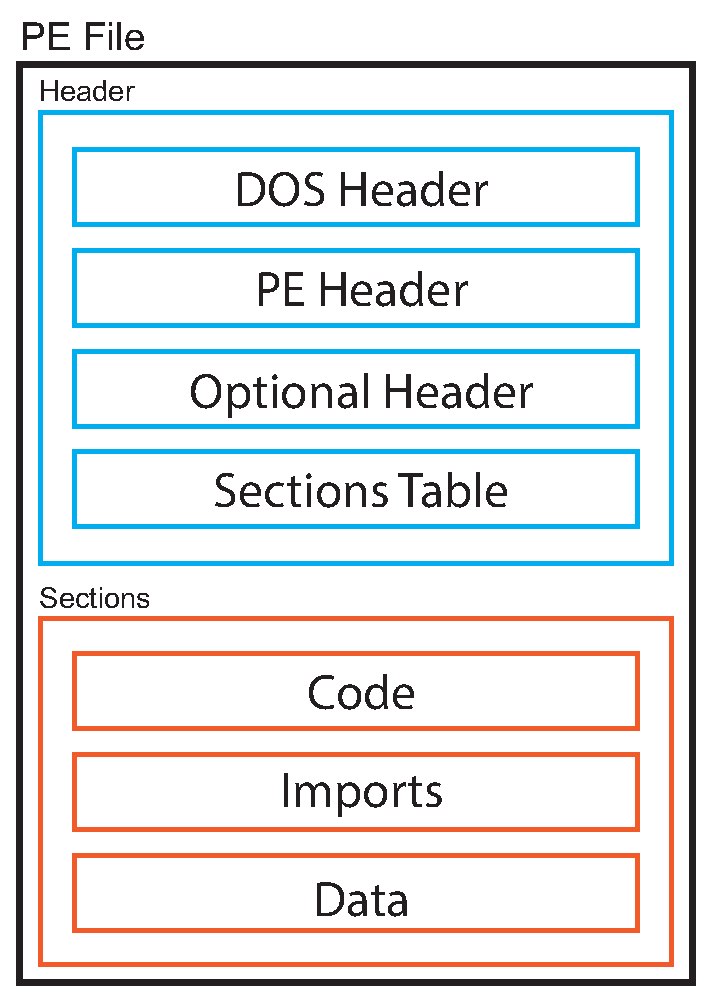
\includegraphics[width=60mm,scale=0.5]{Figures/obrazky/pe-file.eps}
    \label{fig:peformat}
\end{figure}


\paragraph*{Hlavička} Jak už bylo zmíněno, hlavička PE souboru obsahuje celou řadu důležitých metadat pro zavedení aplikace do uživatelského prostoru. Části této hlavičky jsou dále popsány v následujícím textu.

\subparagraph*{DOS Header}
%MSDOS hlavička + program pro dos CANNOT BE RUN IN DOS mode
Prvních 64 bytů souboru ve formátu PE vždy obsahuje program pro zajištění kompatibility s OS MS-DOS. Tento program slouží k upozornění, že se nejedná o aplikaci určenou pro prostředí MS-DOS. Po jeho spuštění se vypíše hláška \emph{This program cannot be run in DOS mode}. První hodnotou této DOS hlavičky je hodnota \emph{e\_magic} (magické číslo - viz \ref{magic_numbers}), které identifikuje DOS mód \cite{Zatloukal2017MalwareDB}. Zároveň tato hlavička obsahuje offset (logická adresa) \emph{e\_lfanew}, jež odkazuje na začátek PE hlavičky \cite{pe_format_history}.

\subparagraph*{PE Header} \ref{peheader_entrypoint}
Po DOS hlavičce následuje PE hlavička. Na offsetu 0x3C se nachází 4 bytový podpis identifikující soubor jako PE formát \cite{Liao2012PEHeaderBasedMS}. Tento podpis odpovídá hodnotě \emph{PE\textbackslash0\textbackslash0} \cite{msdocs_pe}.

\subparagraph*{Optional Header}
Následuje optional header (v překladu volitelná hlavička), která je však volitelná pouze v případě objektových souborů, kde by neměla význam a pouze by zabírala místo. Pro spustitelné EXE soubory a DLL knihovny je tato část povinná \cite{msdocs_pe}, obsahuje totiž důležité informace pro zavaděč jako například entry point (vstupní bod programu označovaný také jako~\emph{EP}) nebo počet sekcí \cite{pe_format_history}. 

\subparagraph*{Sections Table}

Po volitelné hlavičce následuje tabulka sekcí, jež obsahuje hlavičky jednotlivých sekcí spustitelného souboru. Každá hlavička obsahuje název sekce, její velikost, umístění a charakteristiky sekce \cite{infosecinstitute_pe}.

\paragraph*{Sekce}
%An application for Windows NT typically has the nine predefined sections named .text, .bss, .rdata, .data, .rsrc, .edata, .idata, .pdata, and .debug. Some applications do not need all of these sections, while others may define still more sections to suit their specific needs. 
Aplikace pro OS Windows mohou využít 9 předdefinovaných sekcí jako \emph{.text, .bss, .rdata, .data, .rsrc, .edata, .idata, .pdata a .debug} nebo si dle svých potřeb vytvořit vlastní \cite{pe_format_history}. 

Důležité sekce budou popsány níže.

\subparagraph*{Sekce .text}
Tato sekce obsahuje instrukce programu pro procesor, který je následně vykonává. Odkazuje na ni entry point v PE Header (viz \label{peheader_entrypoint}) Často je to jediná sekce, ze které je program spouštěn \cite{sikorski2012practical}.

\subparagraph*{Sekce zdrojových dat (.rsrc)}

Další sekcí je sekce \emph{.rsrc}. Tato sekce obsahuje zdroje (resources) pro běh programu, které nejsou uloženy přímo v programu. Jsou to například obrázky, binární data nebo řetězce, které však mohou být přímo součástí kódu. Tyto sekce jsou často využity kupříkladu v programech, které obsahují více jazykových mutací \cite{sikorski2012practical}.

\subparagraph*{Datové sekce (.bss, .rdata, .data)}

Po sekci zdrojových dat následují sekce datové. Sekce \emph{.bss} (Block Started by Symbol) obsahuje neinicializovaná data aplikace jako statické proměnné apod. V další sekci \emph{.rdata} jsou uložena data určená pouze pro čtení jako globální konstanty atd. \cite{infosecinstitute_pe}. Poslední typ datové sekce je pak sekce \emph{.data}, jež obsahuje globální data, která jsou přístupná z jakékoliv části kódu v aplikaci. \cite{sikorski2012practical}

\subparagraph*{Sekce s exporty (.edata)}

Sekce \emph{.edata} obsahuje informace k exportům jako názvy a~adresy exportovaných funkcí \cite{infosecinstitute_pe}.

\subparagraph*{Sekce s importy (.idata)}

Po sekci s exporty je nutno také zmínit sekci \emph{.idata}, která~naopak obsahuje informace k importům (adresní tabulka importu aj.) \cite{infosecinstitute_pe}. 

%\subparagraph*{Sekce  (.tls)}
%Poslední důležitou sekcí je \emph{.tls} sekce, jež obsahuje

\paragraph*{Nástroje pro analýzu}

Nástrojů pro analýzu spustitelných souborů existuje celá řada. V~následujícím textu budou zmíněny některé z nich. 

\subparagraph*{PEiD}
% detekce packeru, kryptoru, komprese
% vyvoj ukončen 
% pouze PE
% detekce signatur možnost dodat svoje
% https://ieeexplore.ieee.org/abstract/document/4654055 \cite{4654055}

Tento nástroj je jeden z nejpoužívanějších. Je určen pro detekci známých packerů, kryptorů a kompilátorů na základě databáze signatur. V základu obsahuje databázi více než 470 signatur, je však možné přidat i své vlastní. Existují také databáze obsahující přes 3000 signatur, které je možné použít s aplikací PEiD. Detekce pomocí PEiD je ve srovnání s jinými aplikacemi pro detekci packerů velmi dobrá. Obsahuje také rozhraní připravené pro další rozšíření \cite{4654055}. 

Na následujícím obrázku č. \ref{fig:peid} je možné vidět prostředí aplikace PEiD. První část obsahuje základní informace exportované z PE hlavičky jako například, v jaké sekci se nachází entry point nebo jeho offset. Ve spodní části pak lze vidět použitý detekovaný kompilátor nebo packer (viz kapitola \ref{packers}). V našem případě byl detekován packer UPX.

\begin{figure}[!ht]
    \centering
    \caption{Program PEiD}
    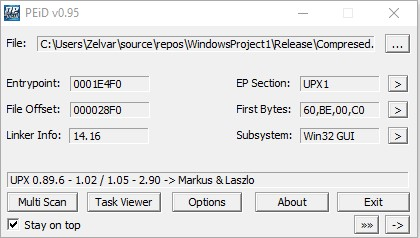
\includegraphics[width=100mm,scale=0.5]{Figures/obrazky/PEid.jpg}
    \label{fig:peid}
\end{figure}

Pod základním výstupem pak nástroj nabízí různé možnosti nastavení jako například přepnutí úrovně skenování. Nabízené možnosti skenování jsou \emph{Normal mode}, který vyhledává signatury okolo EP, \emph{Deep mode} skenuje celou sekci. \emph{Deep mód} detekuje až 80\% souborů, které jsou chráněny před analýzou pomocí packerů. Poslední možností je \emph{Hardcore mode}, který skenuje celý PE soubor na známé signatury \cite{peid_info} což však může trvat výrazně delší dobu.

Nevýhodou tohoto nástroje je, že neumí pracovat s aplikacemi určenými pro platformu x64 (PE32+). Další vývoj již neprobíhá.

\subparagraph*{Exeinfo PE}

Alternativou PEiD může být nástroj Exeinfo, který podporuje také PE32+. Hlavní výhodou je, že vývoj programu stále probíhá (poslední verze vyšla 22.10.2019) \cite{exeinfo}. 

Uživatelské rozhraní je velmi podobné PEiD (viz obrázek č. \ref{fig:exeinfo}), výstup také obsahuje nápovědu s~návodem k~provedení unpackingu (viz kapitola \ref{unpackers}).

Nevýhodou však je to, že program neumí detekovat starší způsoby ochrany (např. packery nebo protektory viz kapitola \ref{packers}) \cite{exeinfo_malwarebytes}.

\begin{figure}[!ht]
    \centering
    \caption{Program Exeinfo PE}
    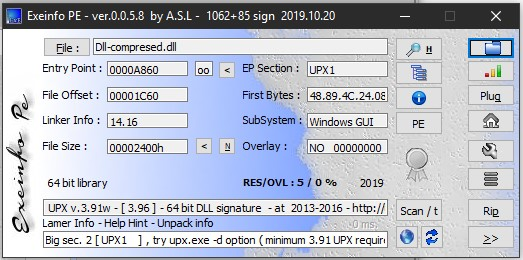
\includegraphics[width=100mm,scale=0.5]{Figures/obrazky/Exeinfo.jpg}
    \label{fig:exeinfo}
\end{figure}


\subparagraph*{PE Studio}

Dalším možným nástrojem pro práci se spustitelným souborem formátu PE je PE Studio. Tento program je nabízen ve dvou variantách, jedna je zdarma a nabízí základní statickou analýzu souboru, a druhá pokročilá je nabízena za poplatek \cite{pestudio}. Na obrázku č. \ref{fig:pestudio} je možné vidět rozhraní tohoto programu (konkrétně jeho bezplatné verze).

Základní verze programu obsahuje běžně nabízené funkce konkurenčními aplikacemi mimo jiné ale také pokročilejší funkce, které nazývá indikátory. Tyto indikátory využívají metody jako je detekce signatur, detekce URL a IP adres v~kódu, vyhledávaní zakázaných řetězců ze slovníku (keyloger apod.), hledání klíčových slov mezi řetězci atp. \cite{exeinfo_malwarebytes}.

Výstup programu je rozdělen chronologicky do několika podoken (viz obrázek č. \ref{fig:pestudio}) dle funkcí. Obsahuje jak již zmíněné indikátory, tak výstup z nástroje VirusTotal, seznam řetězců, seznam sekcí atd.

\begin{figure}[!ht]
    \centering
    \caption{Nástroj PE Studio}
    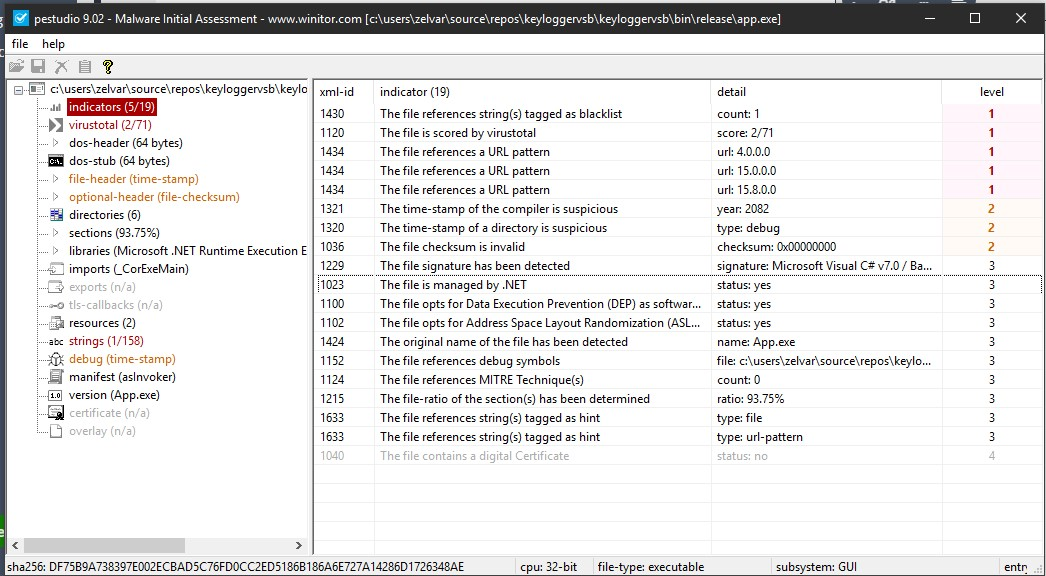
\includegraphics[width=160mm,scale=1]{Figures/obrazky/PeStudio.jpg}
    \label{fig:pestudio}
\end{figure}